
\documentclass[varwidth=\maxdimen, border=0.2cm]{standalone} 
\usepackage[T1]{fontenc}
\usepackage[utf8]{inputenc}
\usepackage{xcolor}
\usepackage{tikz}
\usepackage{tikz-qtree}
\usetikzlibrary{positioning}

\definecolor{bluish}{HTML}{E0EBF5}
\definecolor{yellish}{HTML}{FFFFA8}
\definecolor{dbluish}{HTML}{375EAB}
\definecolor{brownish}{HTML}{BC8C64}
\definecolor{darkish}{HTML}{6F6B69}
\definecolor{darkish2}{HTML}{848475}




\begin{document}

\begin{center}
 {\large\tt let a $=${} 5$/${}2 $=${}$=${} 2} 
\end{center}

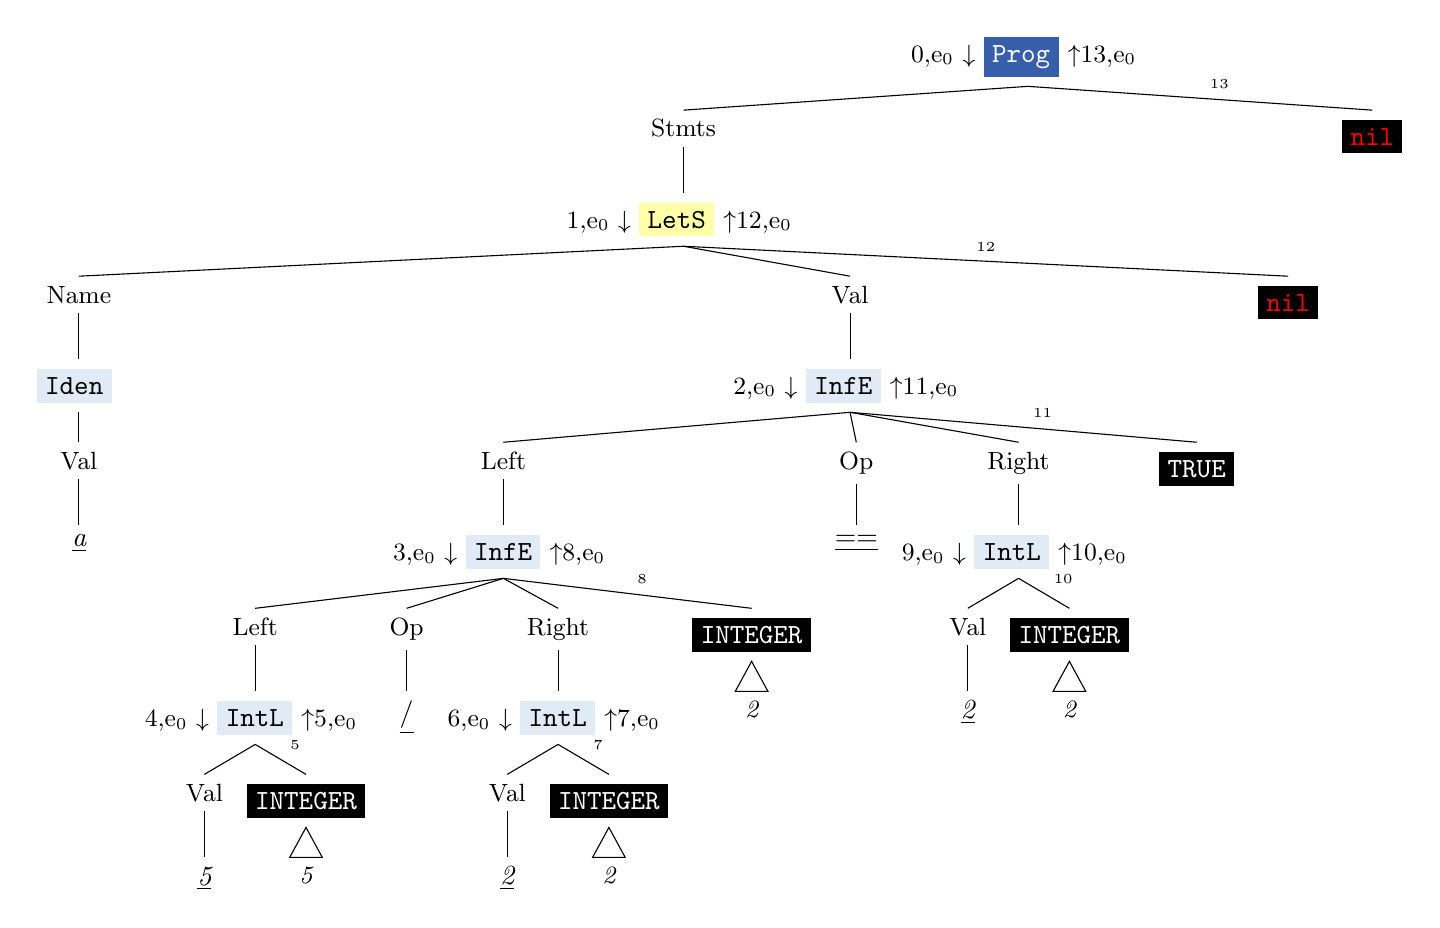
\begin{tikzpicture}[
   every tree node/.style={anchor=north},
   every node/.append style={align=left}  
]

\Tree [.{{\small 0,e$_{0}$ $\downarrow$ }\colorbox{dbluish}{\textcolor{white}{\tt Prog}} {\small  $\uparrow$13,e$_{0}$ }}
  [.{\small Stmts} 
    [.{{\small 1,e$_{0}$ $\downarrow$ }\colorbox{yellish}{\textcolor{black}{\tt LetS}} {\small  $\uparrow$12,e$_{0}$ }}
      [.{\small Name} 
        [.{{\small }\colorbox{bluish}{\textcolor{black}{\tt Iden}} {\small }}
          [.{\small Val} 
            \underline{\it a}
          ]
        ]
      ]
      [.{\small Val} 
        [.{{\small 2,e$_{0}$ $\downarrow$ }\colorbox{bluish}{\textcolor{black}{\tt InfE}} {\small  $\uparrow$11,e$_{0}$ }}
          [.{\small Left} 
            [.{{\small 3,e$_{0}$ $\downarrow$ }\colorbox{bluish}{\textcolor{black}{\tt InfE}} {\small  $\uparrow$8,e$_{0}$ }}
              [.{\small Left} 
                [.{{\small 4,e$_{0}$ $\downarrow$ }\colorbox{bluish}{\textcolor{black}{\tt IntL}} {\small  $\uparrow$5,e$_{0}$ }}
                  [.{\small Val} 
                    \underline{\it 5}
                  ]
                  \edge node[auto=left]{\tiny 5};  [.\colorbox{black}{\textcolor{white}{\tt INTEGER}}
                    \edge[roof];{\small\it 5}
                  ]
                ]
              ]
              [.{\small Op} 
                \underline{\it $/${}}
              ]
              [.{\small Right} 
                [.{{\small 6,e$_{0}$ $\downarrow$ }\colorbox{bluish}{\textcolor{black}{\tt IntL}} {\small  $\uparrow$7,e$_{0}$ }}
                  [.{\small Val} 
                    \underline{\it 2}
                  ]
                  \edge node[auto=left]{\tiny 7};  [.\colorbox{black}{\textcolor{white}{\tt INTEGER}}
                    \edge[roof];{\small\it 2}
                  ]
                ]
              ]
              \edge node[auto=left]{\tiny 8};  [.\colorbox{black}{\textcolor{white}{\tt INTEGER}}
                \edge[roof];{\small\it 2}
              ]
            ]
          ]
          [.{\small Op} 
            \underline{\it $=${}$=${}}
          ]
          [.{\small Right} 
            [.{{\small 9,e$_{0}$ $\downarrow$ }\colorbox{bluish}{\textcolor{black}{\tt IntL}} {\small  $\uparrow$10,e$_{0}$ }}
              [.{\small Val} 
                \underline{\it 2}
              ]
              \edge node[auto=left]{\tiny 10};  [.\colorbox{black}{\textcolor{white}{\tt INTEGER}}
                \edge[roof];{\small\it 2}
              ]
            ]
          ]
          \edge node[auto=left]{\tiny 11};  \colorbox{black}{\textcolor{white}{\tt TRUE}}
        ]
      ]
      \edge node[auto=left]{\tiny 12};  [.\colorbox{black}{\textcolor{red}{\tt nil}} ]
    ]
  ]
  \edge node[auto=left]{\tiny 13};  [.\colorbox{black}{\textcolor{red}{\tt nil}} ]
]
\end{tikzpicture}

\end{document}
